\model{Common Methods}

Classes are often used to represent abstract data types, such as \java{Color} or \java{Point}.
They are also used to represent objects in the real world, such as \java{CreditCard} (see \ref{credit-card.tex}) or \java{Person}.

\begin{center}
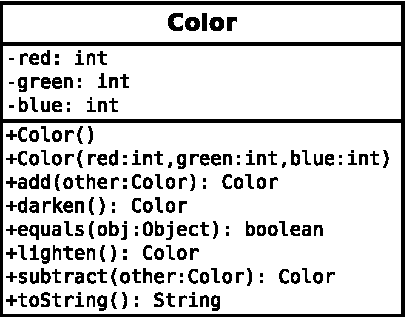
\includegraphics{Color.pdf}  % immutable
~~~~~
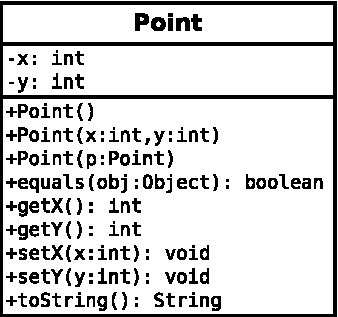
\includegraphics{Point.pdf}  % mutable
\end{center}

Classes generally include the following kinds of methods (in addition to others):
\begin{itemize}[itemsep=0pt]
\item \textbf{constructor} methods that initialize new objects
\item \textbf{accessor} methods (getters) that return attributes
\item \textbf{mutator} methods (setters) that modify attributes
\item \textbf{object} methods such as \java{equals} and \java{toString}
%\item \textbf{utility} methods which are generally static
\end{itemize}


\quest{20 min}


\Q Identify the constructors for the \java{Color} class.
What is the difference between them?
What arguments do they take?

\begin{answer}
There are two constructors: one that takes three integers for the RGB values, and other that takes a Color object. The latter is called a \emph{copy constructor}. Constructors do not return values.
\end{answer}


\Q What kind of constructor does the \java{Point} class have that the \java{Color} class does not?
What is the purpose of such a constructor?

\begin{answer}
The \java{Point} class also has a default constructor, which initializes attributes to their default value (most likely zero).
\end{answer}


\Q Identify an accessor method in the \java{Point} class.

\begin{enumerate}[itemsep=1pt]
\item Which instance variable does it get? \ans{{\tt this.x} or {\tt this.y}}
\item What arguments does the method take? \ans{none}
\item What does the method return? \ans{The value of \java{x} or \java{y}}
\end{enumerate}


\Q Identify a mutator method in the \java{Point} class.

\begin{enumerate}[itemsep=1pt]
\item Which instance variable does it set? \ans{{\tt this.x} or {\tt this.y}}
\item What arguments does the method take? \ans{The value of \java{x} or \java{y}}
\item What does the method return? \ans{nothing}
\end{enumerate}


\Q \label{immutable}
The \java{Color} class does not have accessors or mutators, but it provides methods that return lighter or darker \texttt{Color} objects.
Why do you think the class was designed this way?

\begin{answer}
Other than the constructor, there are no methods that change the \texttt{red}, \texttt{green}, and \texttt{blue} values.
This design makes the class immutable, which means that objects can be reused.
The \java{String} class is also designed this way.
\end{answer}


\vspace{2em}
\hrulefill

\vspace{1ex}
\textit{For the following questions, consider this portion of source code from the \java{Point} class.}
\vspace{1ex}

\begin{javalst}
    public Point() {
        this.x = 0;
        this.y = 0;
    }

    public boolean equals(Object obj) {
        if (obj instanceof Point) {
            Point p = (Point) obj;
            return this.x == p.x && this.y == p.y;
        }
        return false;
    }

    public String toString() {
        return String.format("(%d, %d)", this.x, this.y);
    }
\end{javalst}

%\hrulefill
%\vspace{1em}


\Q \label{expr}
What is the value of each expression below? (Don't just guess; read the source code above.)
\begin{javalst}
Point p1 = new Point();  Point p2 = new Point(0, 0);  Point p3 = new Point(3, 3);
\end{javalst}

\begin{multicols}{2}
\begin{enumerate}
\item \java{p1 == p1} \ans{true}
\item \java{p1.equals(p1)} \ans{true}
\item \java{p1 == p2} \ans{false}
\item \java{p1.equals(p2)} \ans{true}
\item \java{p1.equals(p3)} \ans{false}
\item \java{p2.toString()} \ans{"(0, 0)"}
\item \java{p2.equals("(3, 3)")} \ans{false}
\item \java{p3.equals("(3, 3)")} \ans{false}
\end{enumerate}
\end{multicols}


\Q What is the purpose of the \texttt{equals} and \texttt{toString} methods?

\begin{answer}[5em]
The \java{equals} method determines whether two objects have the same attribute values, and the \java{toString} method returns a \texttt{String} representation of the \texttt{Point} object.
These methods make it easier to work with user-defined data types.
\end{answer}


\Q What is the purpose of the \java{if}-statement in the \texttt{equals} method?

\begin{answer}
Since \java{equals} can take any type of \java{Object}, you need to check if the argument is a \java{Point} instance before using it as such.
\end{answer}


\Q How could you modify the \java{equals} method to cause both \ref{expr}d and \ref{expr}h to return \java{true}?

\begin{answer}[5em]
Change the last line to ~\texttt{return this.toString().equals(obj);}

You could instead add ~\texttt{if (obj instanceof String)}, but since the \texttt{String.equals} method takes an \texttt{Object}, there's no need to convert the \java{obj} parameter before calling \texttt{String.equals}.
\end{answer}
